La figura~\figref{fig:FTTH_general} muestra la arquitectura general de una red FTTH típica. En la CO (también denominada cabecera), la red de telefonía pública conmutada (PSTN) y los servicios de Internet se interconectan con la red de distribución óptica (ODN) mediante el terminal de línea óptica (OLT). Las longitudes de onda descendentes de 1490 nm y ascendentes de 1310 nm se utilizan para transmitir datos y voz. Los servicios de vídeo RF analógicos se convierten en formato óptico a la longitud de onda 1550 nm mediante el transmisor de vídeo óptico. Las longitudes de onda de 1550 nm y 1490 nm son combinadas por el acoplador WDM y se transmiten juntas de forma descendente. IPTV se transmite sobre 1490 nm.



\begin{wrapfigure}[12]{l}{0.55\textwidth}
  \begin{center}
   	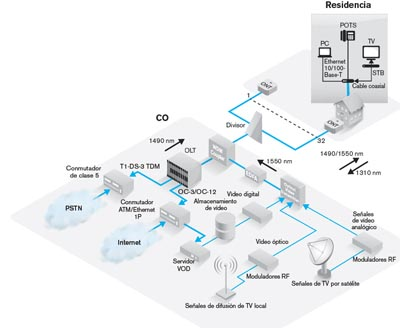
\includegraphics[width=0.55\textwidth]{./img/punto2/Arquitectura-FTTH-general.jpg}	
   	\caption{Arquitectura FTTH general}
	\label{fig:FTTH_general}
  \end{center}  
\end{wrapfigure}


En resumen, las tres longitudes de onda (1310, 1490 y 1550 nm) transportan simultáneamente diferente información y en varias direcciones sobre la misma fibra. El cable de entrada F1 transporta las señales ópticas entre la CO y el divisor, lo cual permite conectar varios ONT a la misma fibra de entrada. Se requiere un ONT para cada abonado y proporciona conexiones para los distintos servicios (voz, datos y vídeo).\\ \\


\vspace{1cm}


Dado que un OLT presta servicio hasta un número de 32 abonados (más de 64 con GPON), normalmente se necesitan muchos OLTs que salgan de la misma CO para servir a una comunidad. Hay diferentes arquitecturas para conectar abonados a la PON. La más sencilla utiliza un divisor único (véase la figura~\figref{fig:Arq_one_layer}), pero también pueden emplearse varios divisores (véase la figura~\figref{fig:Arq_two_layers}).


\begin{figure}[H]
	\centering
	\includegraphics[width=0.80\textwidth]{./img/punto2/Arquitectura-de-etapa-única.jpg}
	\caption{Arquitectura de etapa única}
	\label{fig:Arq_one_layer}
\end{figure}



\begin{figure}[H]
	\centering
	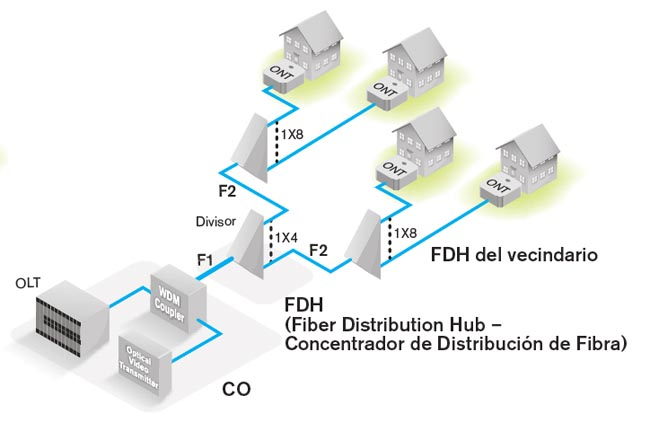
\includegraphics[width=0.80\textwidth]{./img/punto2/Arquitectura-de-dos-etapas.jpg}
	\caption{Arquitectura de dos etapas}
	\label{fig:Arq_two_layers}
\end{figure}





